\documentclass{article} % Класс печатного документа

\usepackage{hyperref} % Для вставки гиперссылок
\usepackage{listings} % Для вставки кусков кода
\usepackage{graphicx} % Вставка изображений
\usepackage[utf8]{inputenc} % Кодировка исходного текста - utf8
\usepackage[english,russian]{babel} % Поддержка языка - русского с английским
\usepackage{indentfirst} % Отступ в первом абзаце

\title{Отчёт 2\protect\\Кластеризация. Метод <<k-средних>>} % Заголовок документа
\author{Свичкарев А.\,В.} % Автор документа
\date{\today} % Текущая дата

\begin{document} % Конец преамбулы, начало текста

\maketitle % Печатает заголовок, список авторов и дату

\section{Цель}
Изучить способы решения задач поиска кластеров в данных.

\section{Задание №1}
Написать программу формирования данных случайных кластеров и их кластерного
анализа по алгоритму <<к-средних>>. Визуализировать в виде графика и сохранить файл
изображения графика кластеров.

Реализация взята из Приложения, произведён рефакторинг и разобран алгоритм.

\clearpage

Кластеризация для выборки из
равномерного распределения
с указанным числом кластеров, равным 3:

\noindent\makebox[\textwidth]{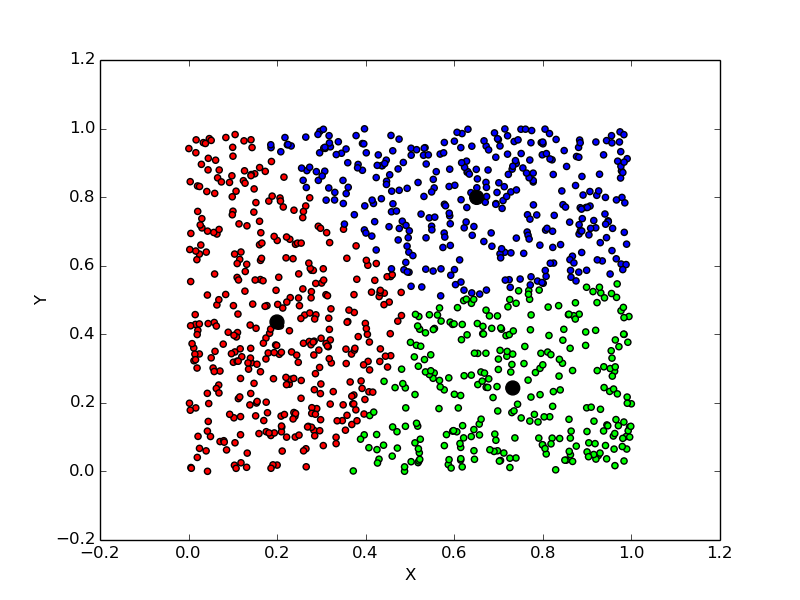
\includegraphics[width=0.7\paperwidth]{Figure_1}}

\clearpage

Кластеризация для двух выборок
из нормальных распределений
с несовпадающими математическими ожиданиями
и дисперсией равной 2:

\noindent\makebox[\textwidth]{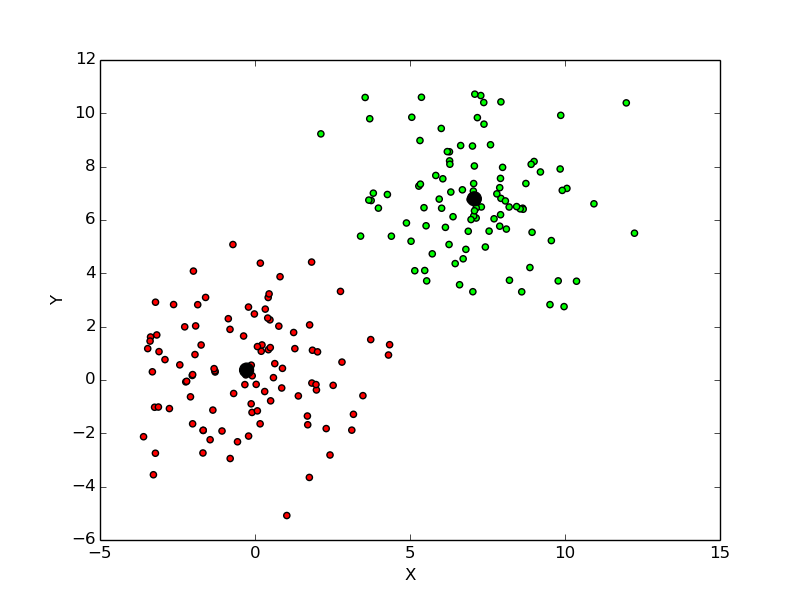
\includegraphics[width=0.7\paperwidth]{Figure_2}}

В секции Исходный код представлена реализация.

\section{Задание №2}

Написать программу кластеризации с определе6нием оптимального числа кластеров \(‘jump’ method\).

Реализация взята из Приложения, произведён рефакторинг и разобран алгоритм.

\clearpage

Кластеризация для трёх выборок
из нормального распределения
со смещёнными математическими ожиданиями
и равными дисперсиями:

\noindent\makebox[\textwidth]{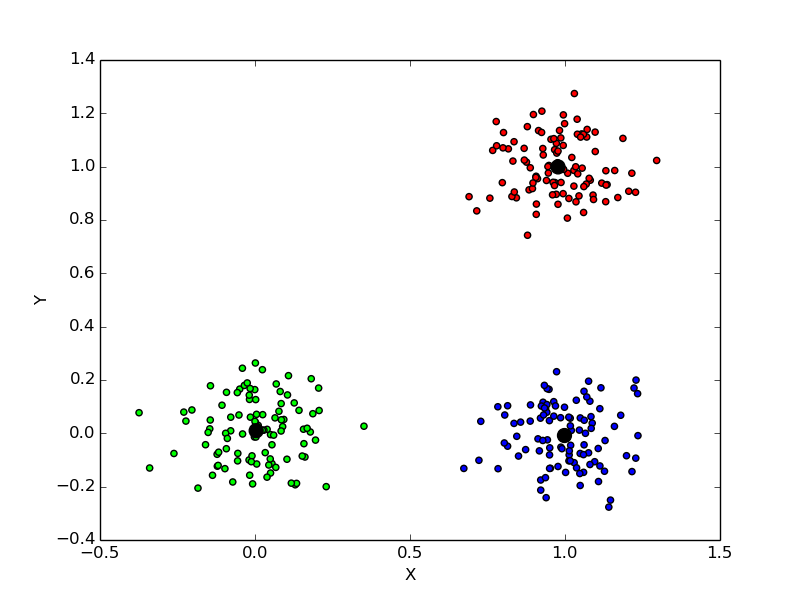
\includegraphics[width=0.7\paperwidth]{Figure_3}}

Для выборки не указывалось число кластеров,
использовался метод описанный в
[Sugar C.A., James G.M. (2003).
Finding the number of clusters in a data set: an information theoretic approach.
Journal of the American Statistical Association 98: 750–763.],
который посчитал оптимальным 3 кластера,
что для этой выборки отражает истинную структуру.

В секции Исходный код представлена реализация.

\section{Выводы}

Алгоритм k-средних способен к <<адаптации>> к данным,
однако очень сильно зависит от начального размещения центров кластеров
для нетривиальных выборок.
К недостаткам также можно отнести необходимость знания числа кластров.
Существует модификация алгоритма,
для которой не нужно указывать число кластеров,
однако этот алгоритм основан на большом числе
тестовых запусков для разных k из диапазона
и выбора оптимального k, используя
среднее удаление элементов данных от центров кластеров
по всем кластрерам.
Такая версия алгоритма работает достаточно долго
в отличие от Иерархической кластеризации,
где выбор числа кластеров можно производить,
анализирую дендрограмму.
Минусом иерархической кластеризацией относительно
кластеризации k-средних можно считать привязку
кластеров к начальным центрам расширения кластеров.

\section{Пояснение}
Исходный код доступен по ссылке:
\href{https://github.com/SvichkarevAnatoly/Course-Python-Bioinformatics/tree/master/semester2/task2}
{github.com}

\section{Исходный код}
Файл \verb$example.py$:
\lstinputlisting[language=Python]{../example.py}

\end{document} % Конец документа
